%! Author = Philipp Emmenegger
%! Date = 29/06/2021

\section{Summary}
\subsection{Guiding Principles}
\begin{enumerate}
    \item Secure the weakest link
    \item Practice defense in depth
    \item Fail securely
    \item Follow the principles of least privilege
    \item Compartmentalize
    \item Keep it simple
    \item Promote privacy
    \item Remember that hiding secrets is hard
    \item Be reluctant to trust
    \item Use your community resources
\end{enumerate}

\subsection{Secure SDLC}
How to address security in the software engineering process
\begin{itemize}
    \item Enriching it with activities for security
    \item Embracing state-of-the-art techniques
\end{itemize}

\subsection{Threat Modeling}
\textbf{DevOps:} Continous Security NOT Security on top or after the fact.\\
\begin{itemize}
    \item Prepare the organization
    \item Protect the software
    \item Produce well secured software
    \item Respond to vulnerabilities
\end{itemize}
\subsubsection{WHY?}
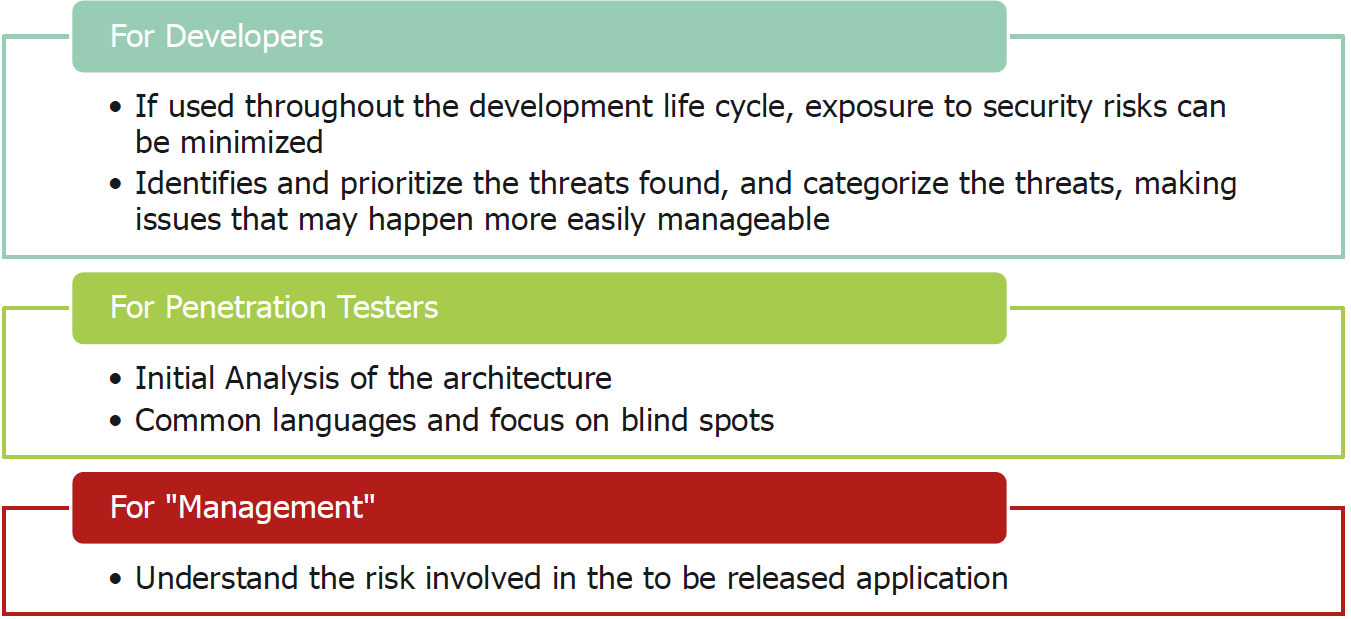
\includegraphics[width=\linewidth]{../img/threat_modeling.png}


